%%
%% Class homework & solution template for latex
%% Alex Ihler
%%
\documentclass[twoside,11pt]{article}
\usepackage{amsmath,amsfonts,amssymb,amsthm}
\usepackage{graphicx,color}
\usepackage{verbatim,url}
\usepackage{listings}
\usepackage{upquote}
\usepackage[T1]{fontenc}
%\usepackage{lmodern}
\usepackage[scaled]{beramono}
\usepackage{enumerate}
%\usepackage{textcomp}

% Directories for other source files and images
\newcommand{\bibtexdir}{../bib}
\newcommand{\figdir}{figs}

\newcommand{\E}{\mathrm{E}}
\newcommand{\Var}{\mathrm{Var}}
\newcommand{\N}{\mathcal{N}}
\newcommand{\matlab}{{\sc Matlab}\ }

\setlength{\textheight}{9in} \setlength{\textwidth}{6.5in}
\setlength{\oddsidemargin}{-.25in}  % Centers text.
\setlength{\evensidemargin}{-.25in} %
\setlength{\topmargin}{0in} %
\setlength{\headheight}{0in} %
\setlength{\headsep}{0in} %

\renewcommand{\labelenumi}{(\alph{enumi})}
\renewcommand{\labelenumii}{(\arabic{enumii})}

\theoremstyle{definition}
\newtheorem{MatEx}{M{\scriptsize{ATLAB}} Usage Example}

\definecolor{comments}{rgb}{0,.5,0}
\definecolor{backgnd}{rgb}{.95,.95,.95}
\definecolor{string}{rgb}{.2,.2,.2}
\lstset{language=Matlab}
\lstset{basicstyle=\small\ttfamily,
        mathescape=true,
        emptylines=1, showlines=true,
        backgroundcolor=\color{backgnd},
        commentstyle=\color{comments}\ttfamily, %\rmfamily,
        stringstyle=\color{string}\ttfamily,
        keywordstyle=\ttfamily, %\normalfont,
        showstringspaces=false}
\newcommand{\matp}{\mathbf{\gg}}




\begin{document}

\centerline{\Large Kyle Benson}
\centerline{CS 273A - Machine Learning: Fall 2013}
\centerline{Homework 1}

% % % % % % % % % % % % % % % % % % % % % % % % % % % % % % % % % % % % % % % % % % % % % % % % % % % % %
\subsection*{Problem 3: }

\begin{enumerate}[(a)]
\item There are 4 features and 148 data points.
\item Histograms of the 4 features:
\begin{figure}[h!] \centering
\begin{tabular}{cccc}
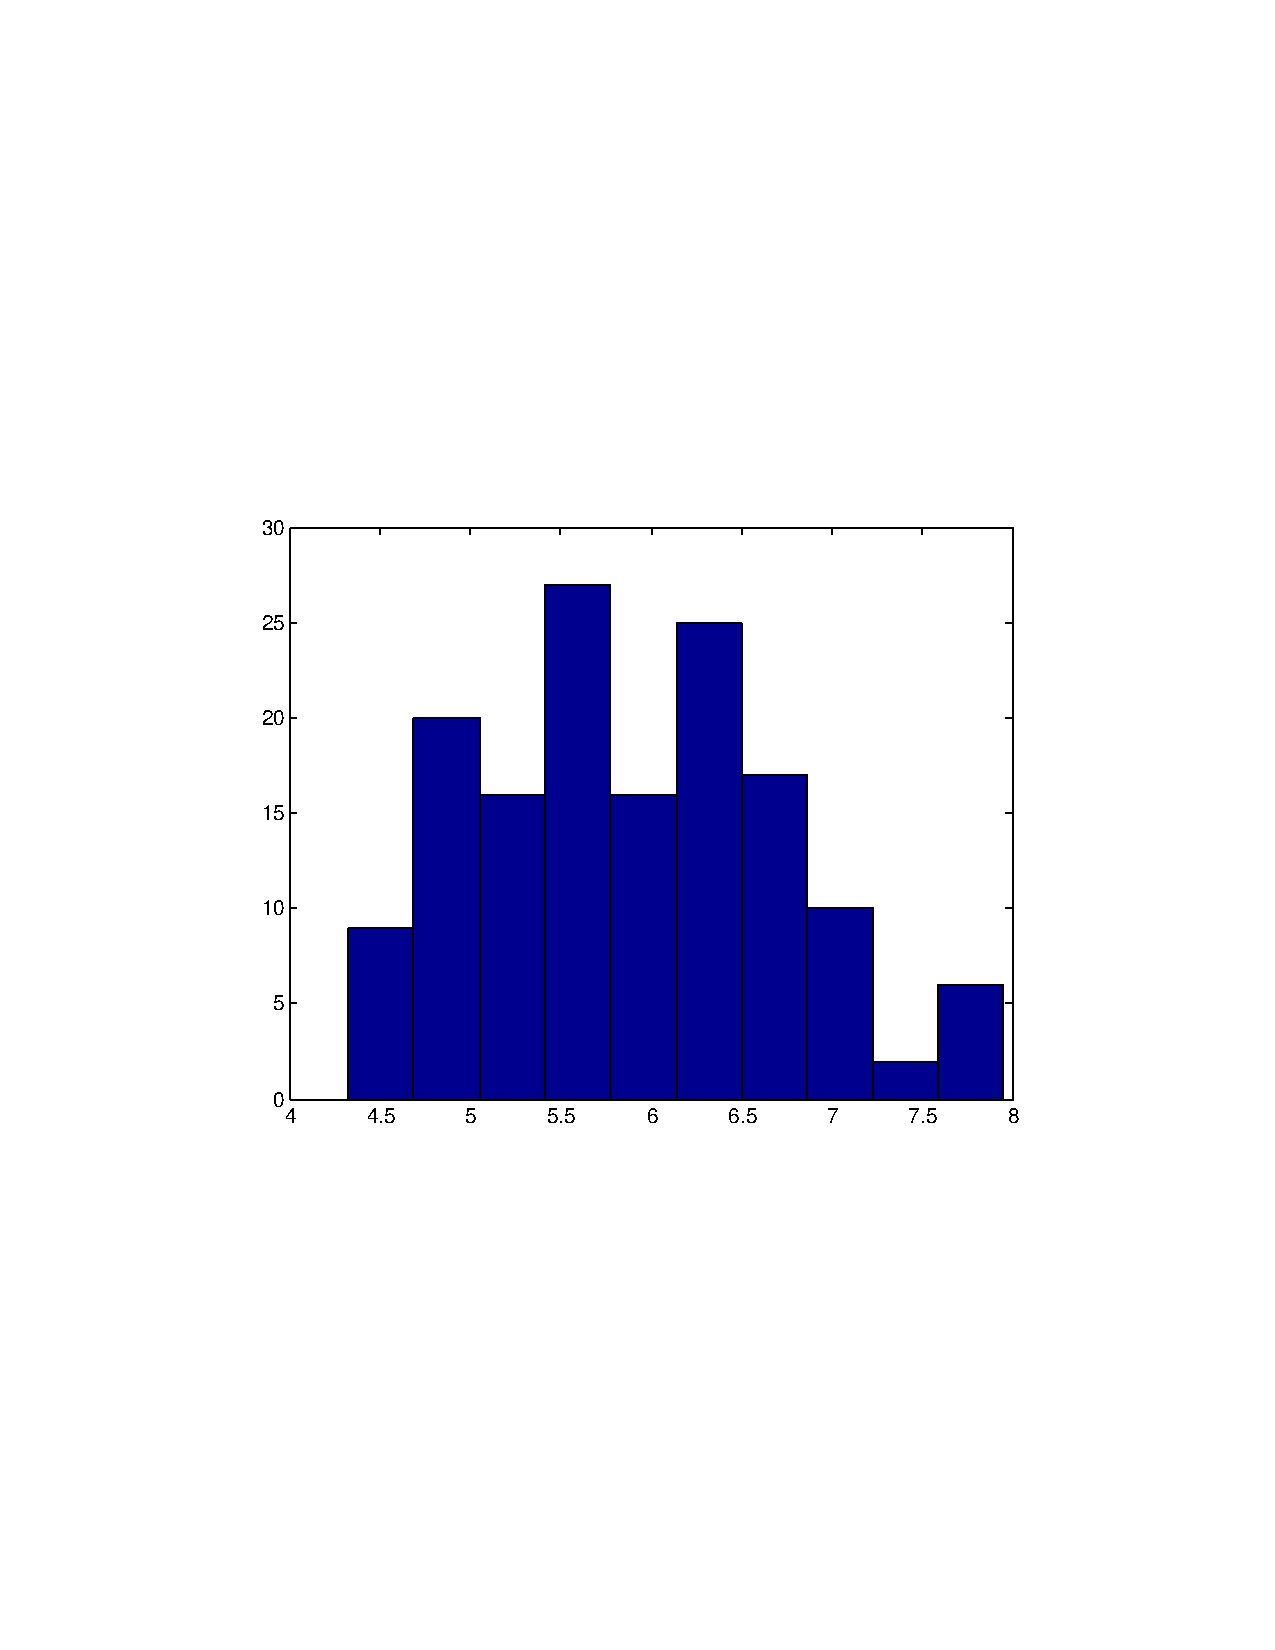
\includegraphics[width=.22\textwidth]{\figdir/iris-feature1} &
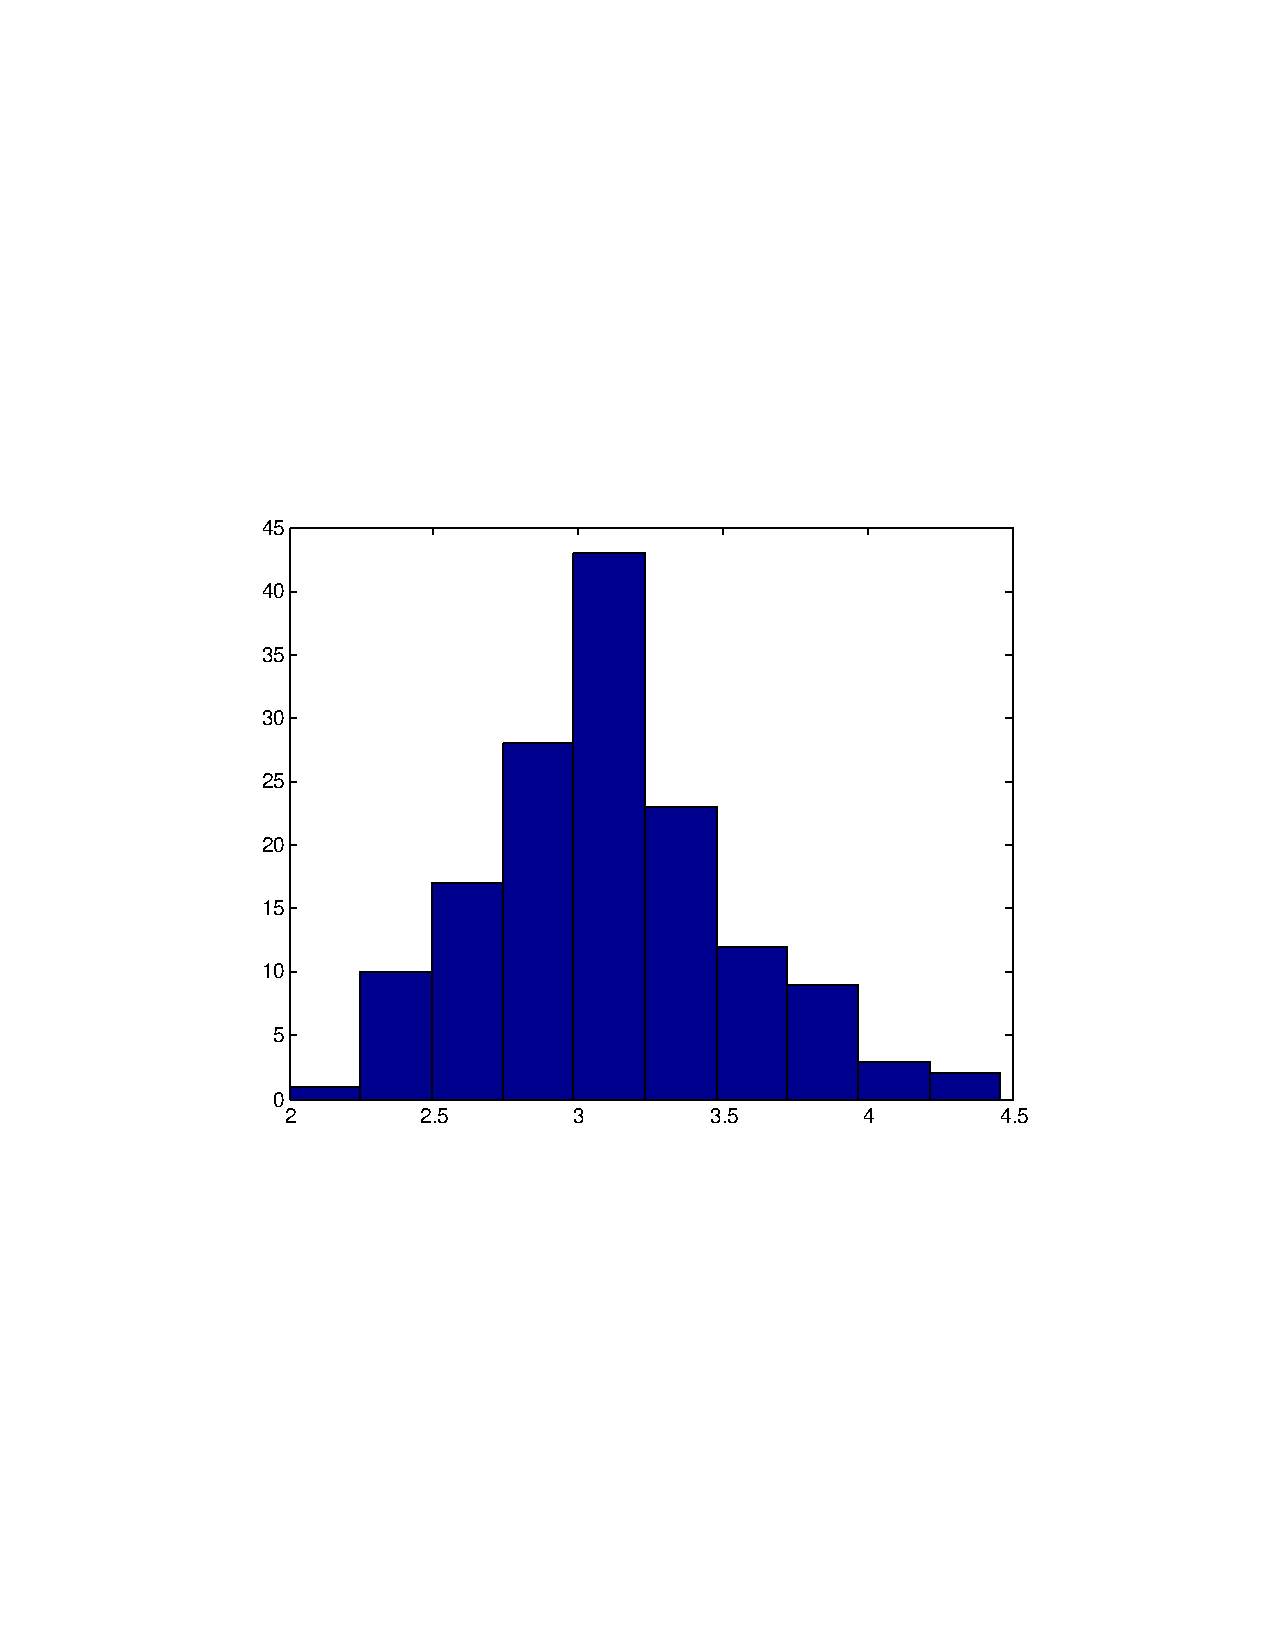
\includegraphics[width=.22\textwidth]{\figdir/iris-feature2} &
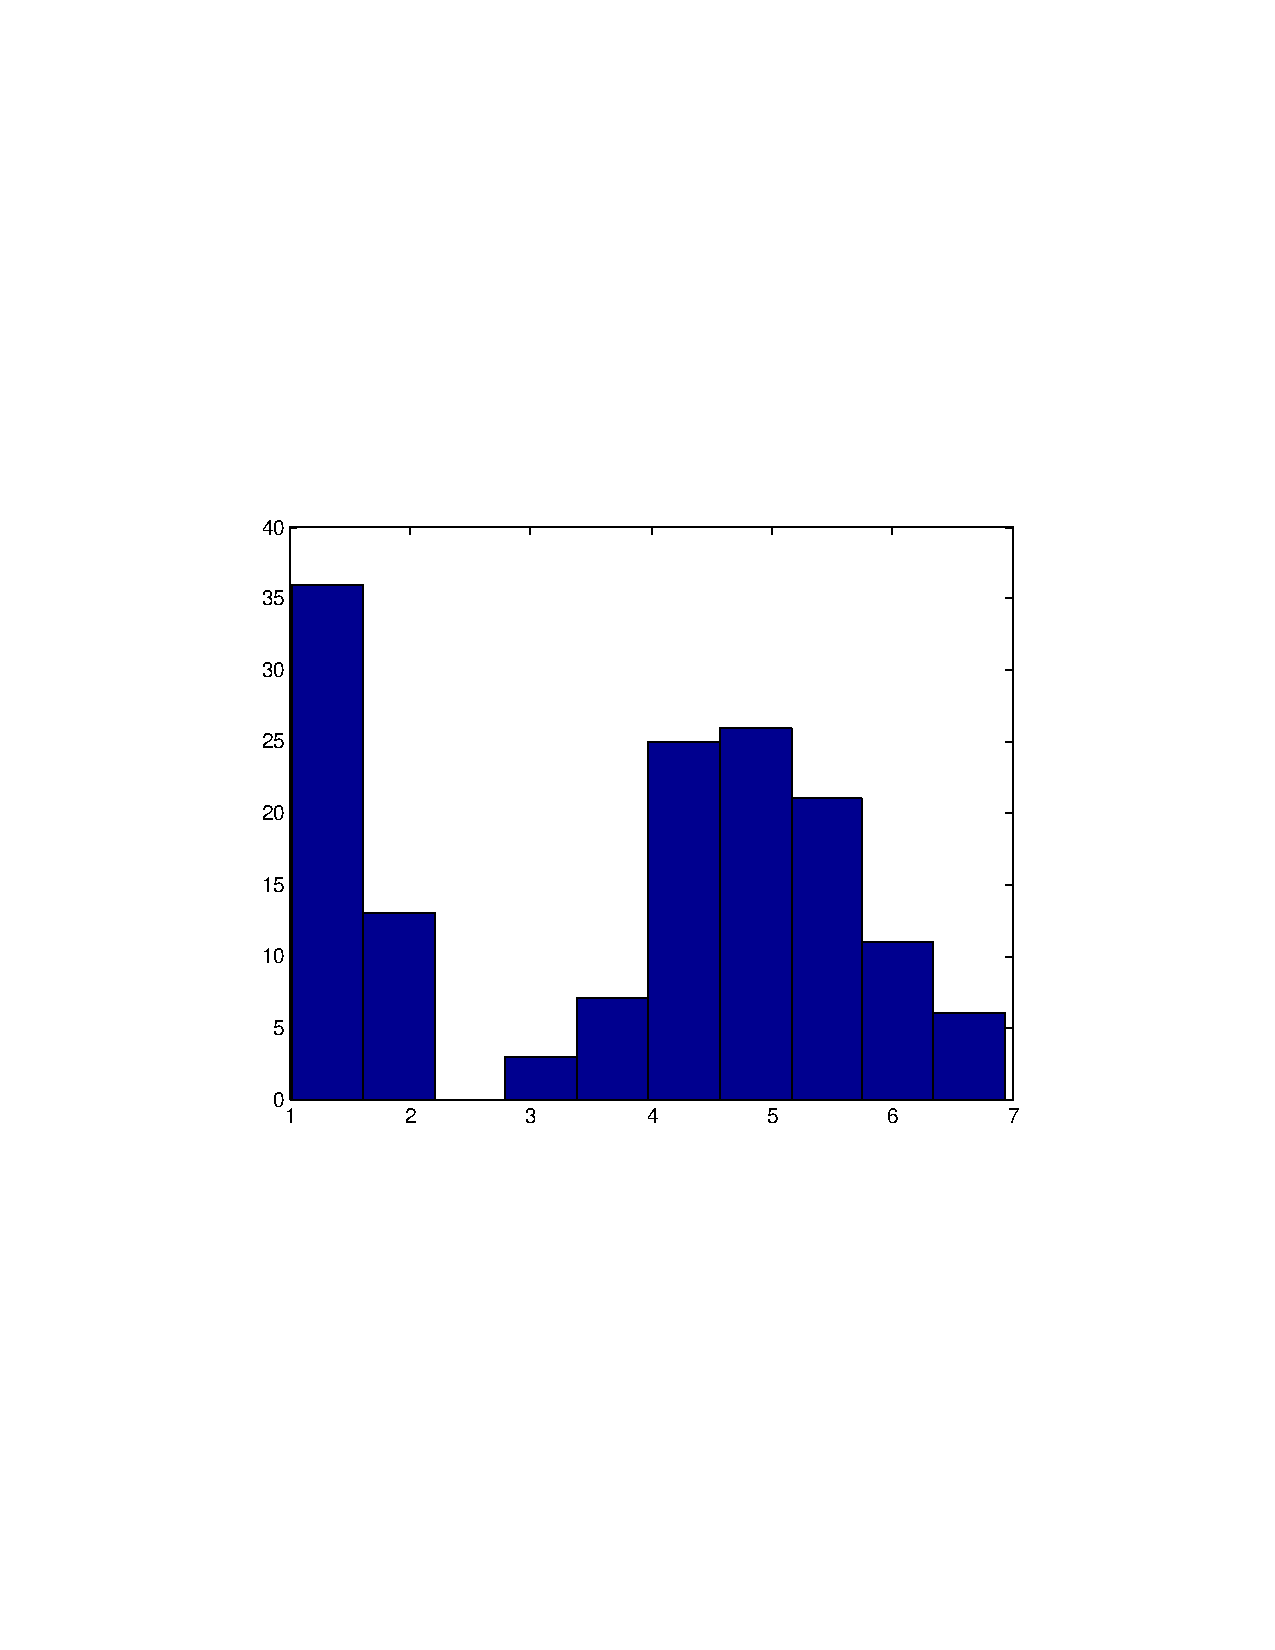
\includegraphics[width=.22\textwidth]{\figdir/iris-feature3} &
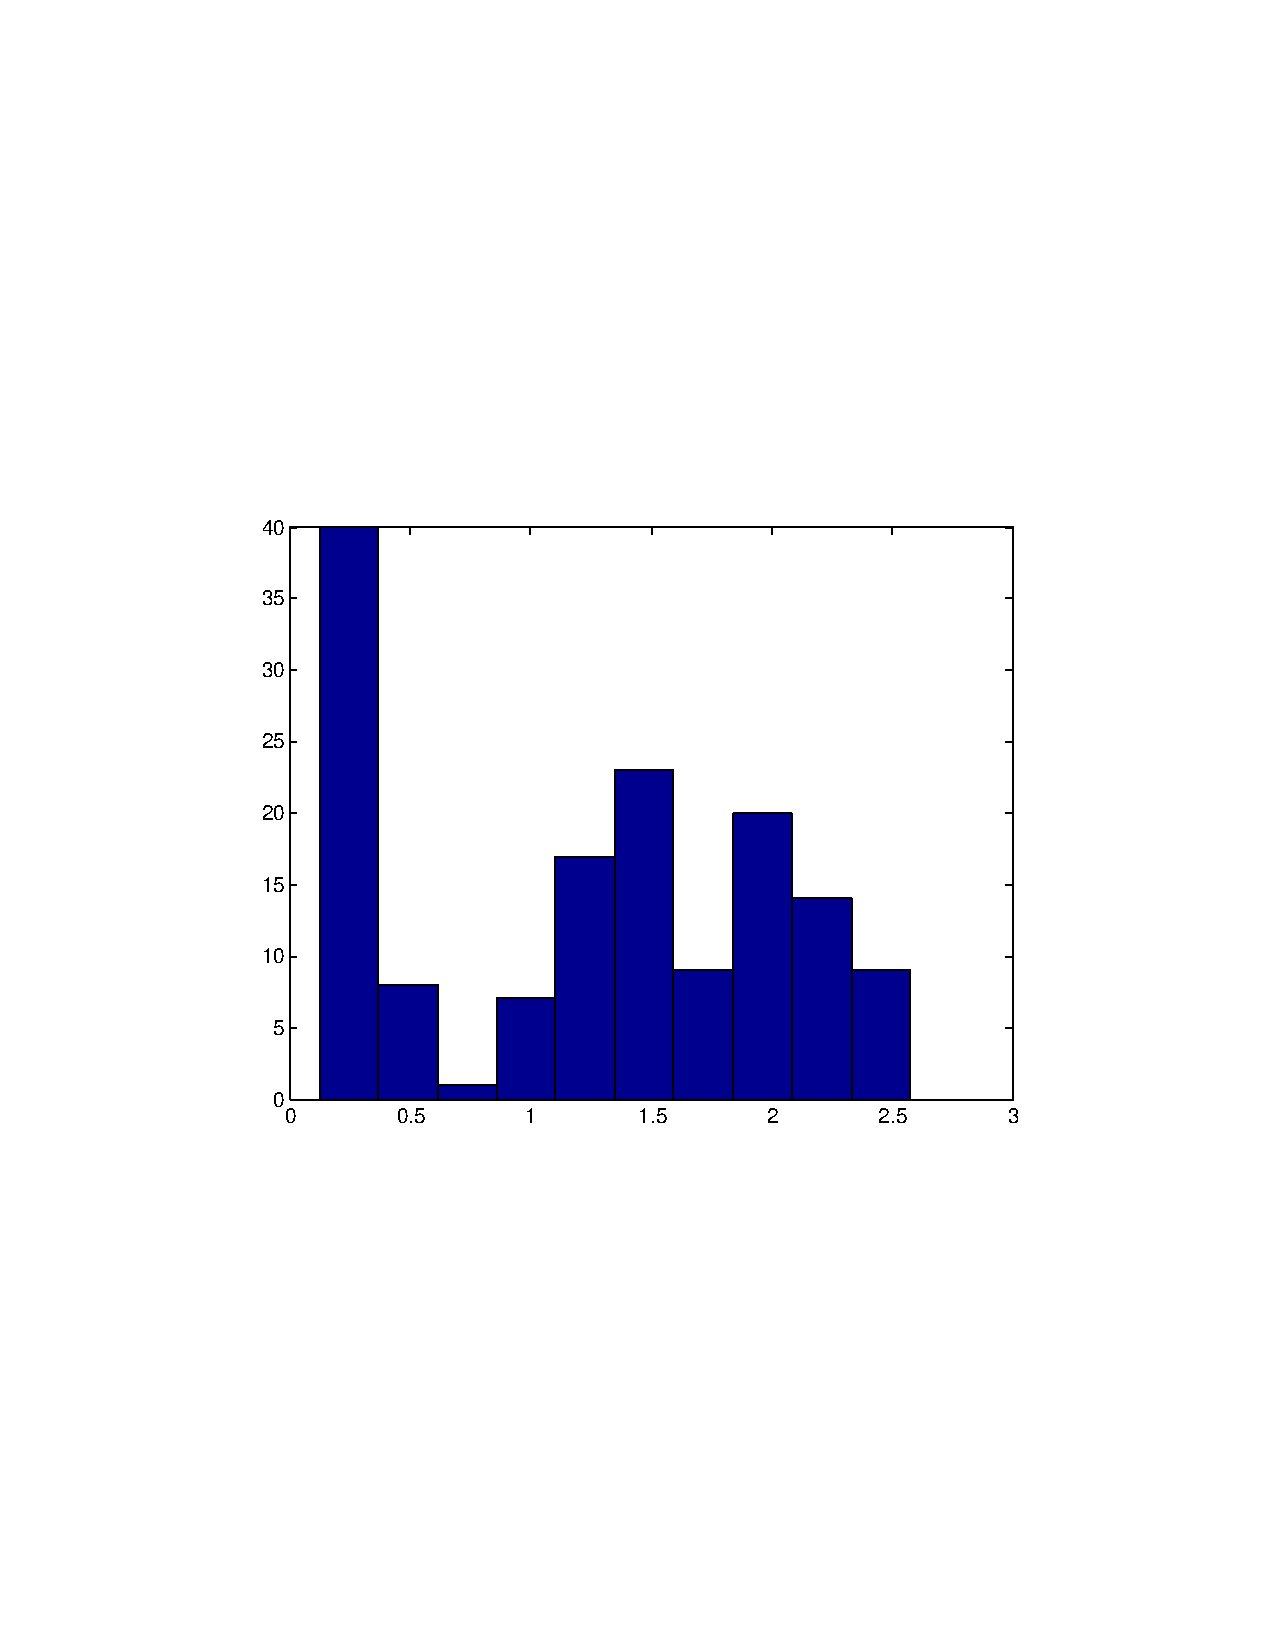
\includegraphics[width=.22\textwidth]{\figdir/iris-feature4} \\
First & Second & Third & Fourth
\end{tabular}
\end{figure}

\item Calling \texttt{mean} on each column gives the following values:\\
\begin{tabular}{ccccc}
feature & one & two & three & four \\
mean &
5.9001 &
3.0989 &
3.8196 &
1.2526 \\
\end{tabular}

\item Calling \texttt{var} and \texttt{stdev} on each feature gives:\\
\begin{tabular}{ccccc}
feature & one & two & three & four \\
variance &
0.6993 &
0.1916 &
3.0976 &
0.5797 \\
stdev &
0.8362 &
0.4378 &
1.7600 & 
0.7613 \\
\end{tabular}

\item I used the following code to store the normalized data in \texttt{d.norm\_data}:\\
\begin{lstlisting}
 d.data = iris(:,1:end-1);     % extract data
 d.mean = mean(d.data)
 d.stdev = std(d.data)
 d.norm_data = bsxfun(@minus, d.data, d.mean) % subtract mean
 d.norm_data = bsxfun(@rdivide, d.norm_data, d.stdev) % divide by stdev
\end{lstlisting}

\item Using different values in the line \\
\texttt{scatter(iris(iris(:,5)==target,1), iris(iris(:,5)==target,feat), [color '.'])},
I got the following plots:
\begin{figure}[h!] \centering
\begin{tabular}{ccc}
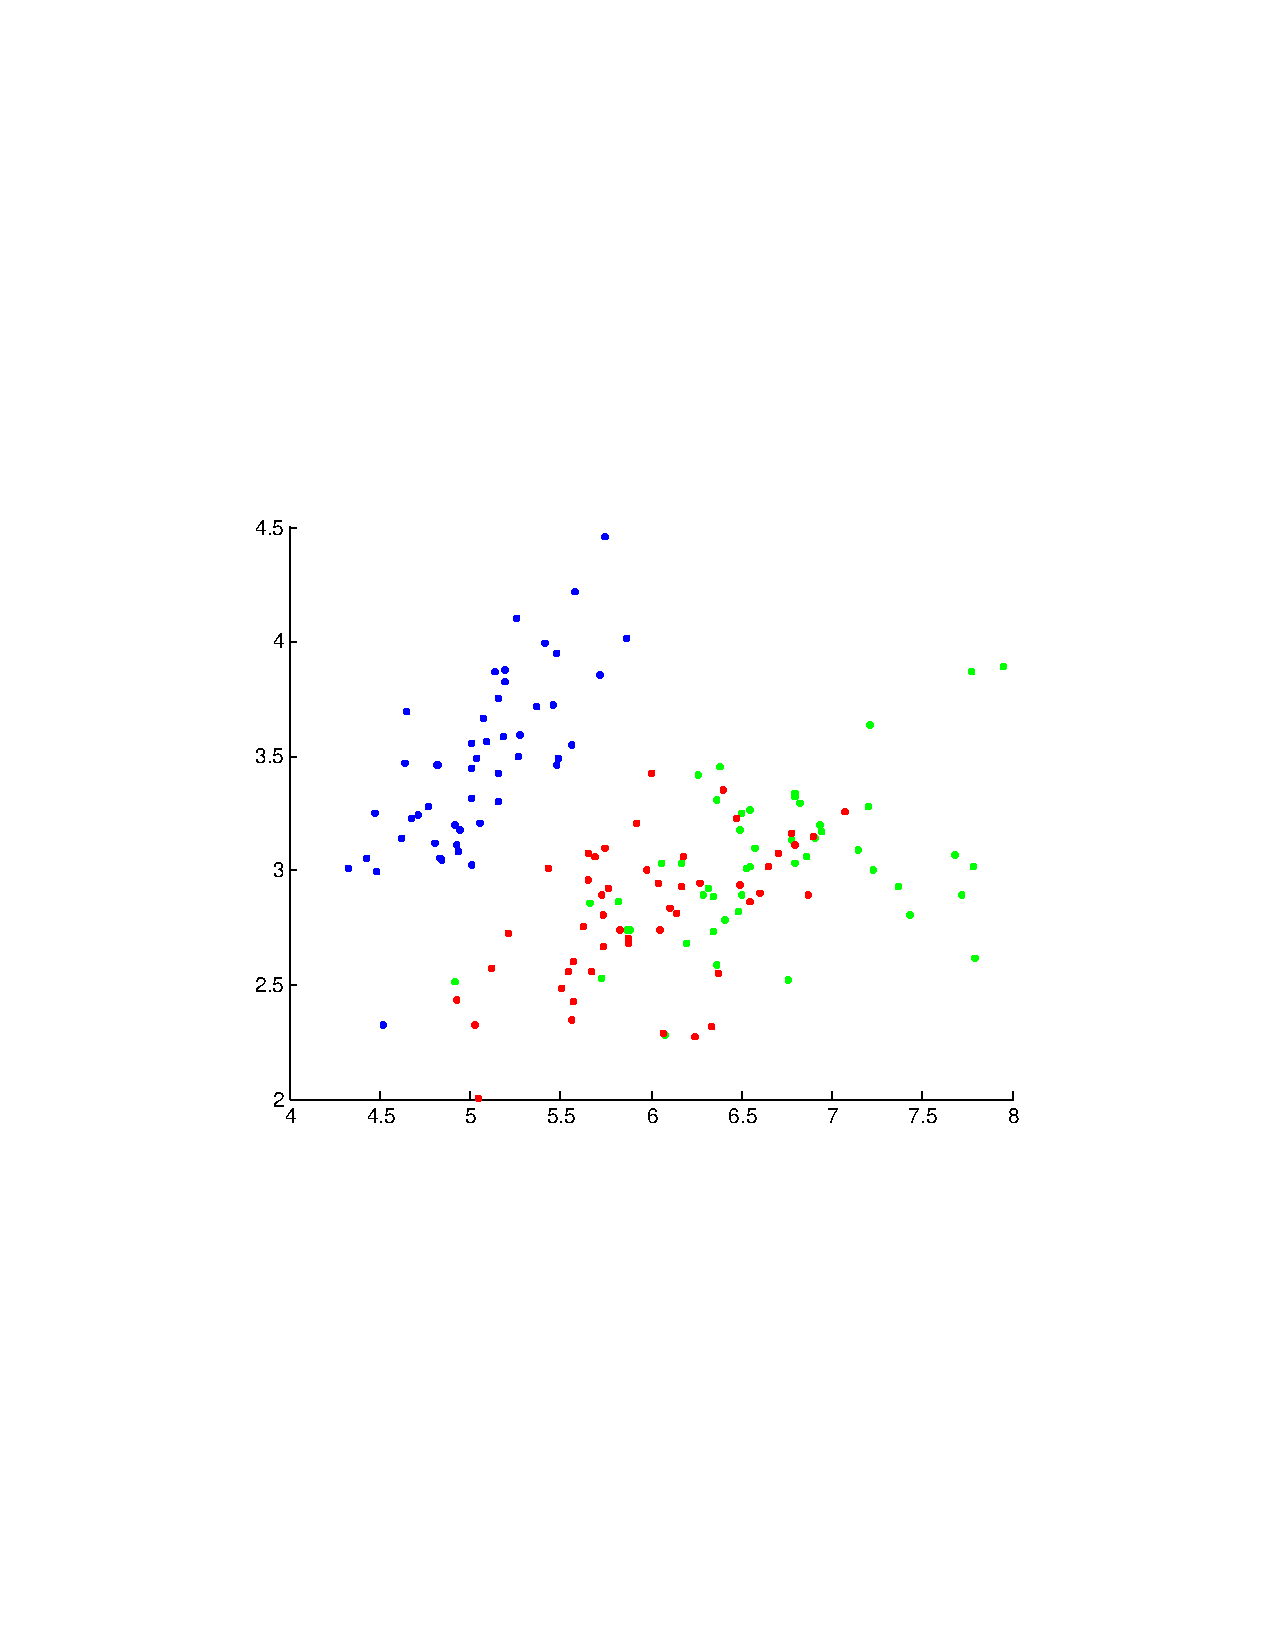
\includegraphics[width=.22\textwidth]{\figdir/iris-feature-scatter-1v2} &
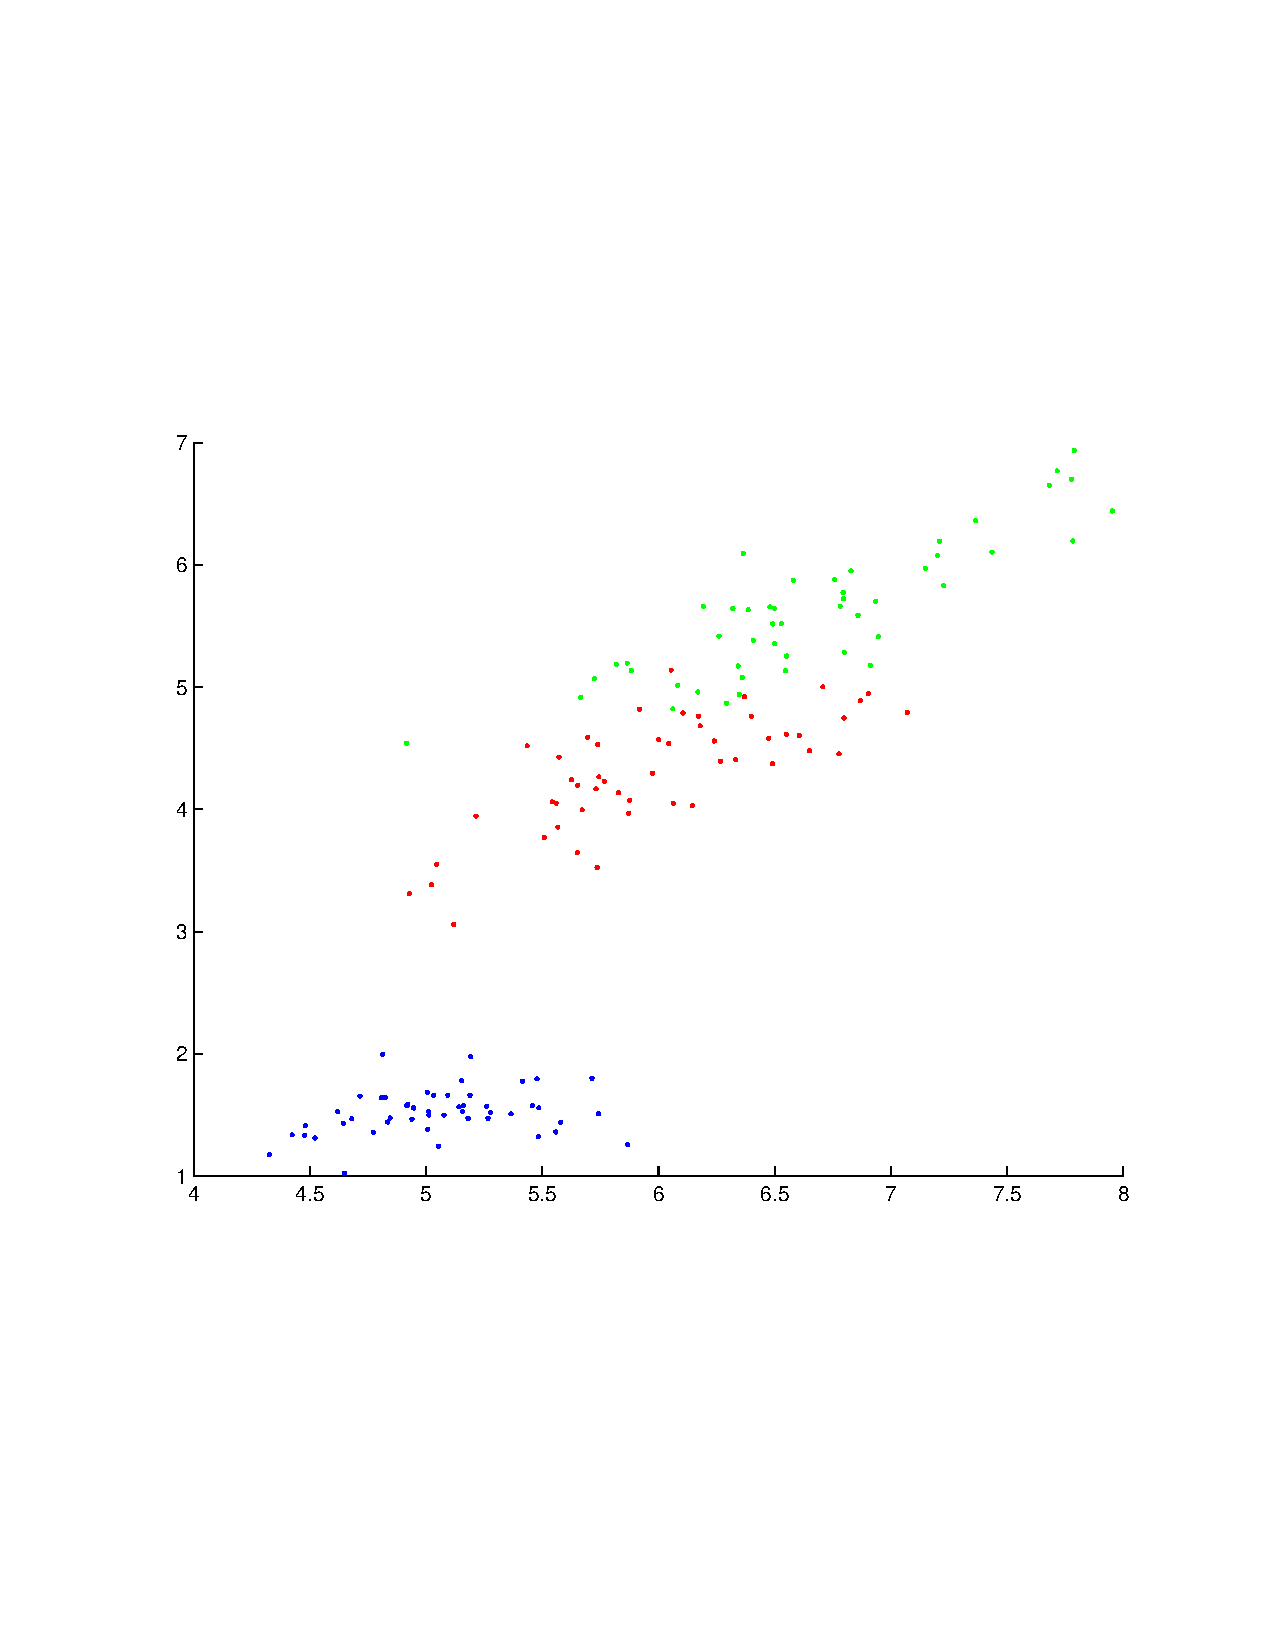
\includegraphics[width=.22\textwidth]{\figdir/iris-feature-scatter-1v3} &
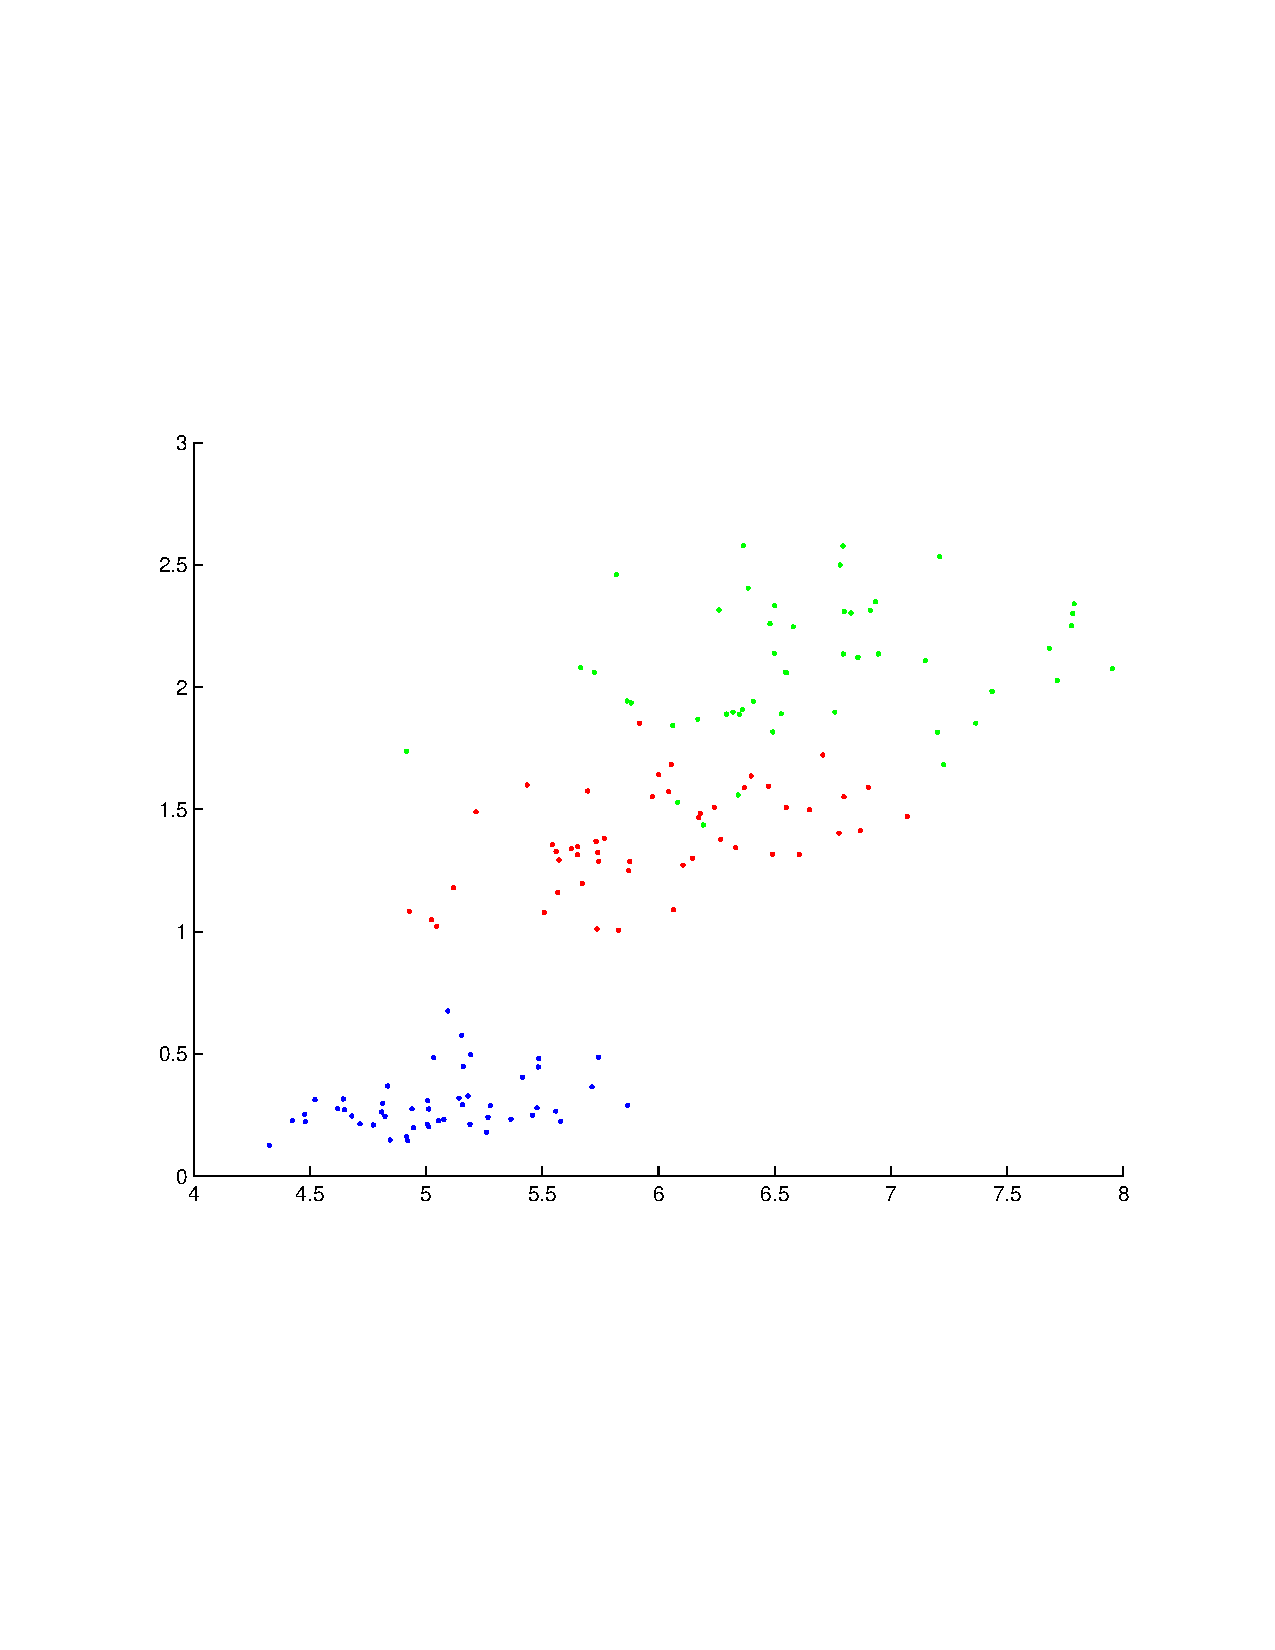
\includegraphics[width=.22\textwidth]{\figdir/iris-feature-scatter-1v4} \\
1v2 & 1v3 & 1v4
\end{tabular}
\end{figure}
\end{enumerate}

% % % % % % % % % % % % % % % % % % % % % % % % % % % % % % % % % % % % % % % % % % % % % % % % % %

\subsection*{Problem 4: }

Following the given steps gives this plot:\\
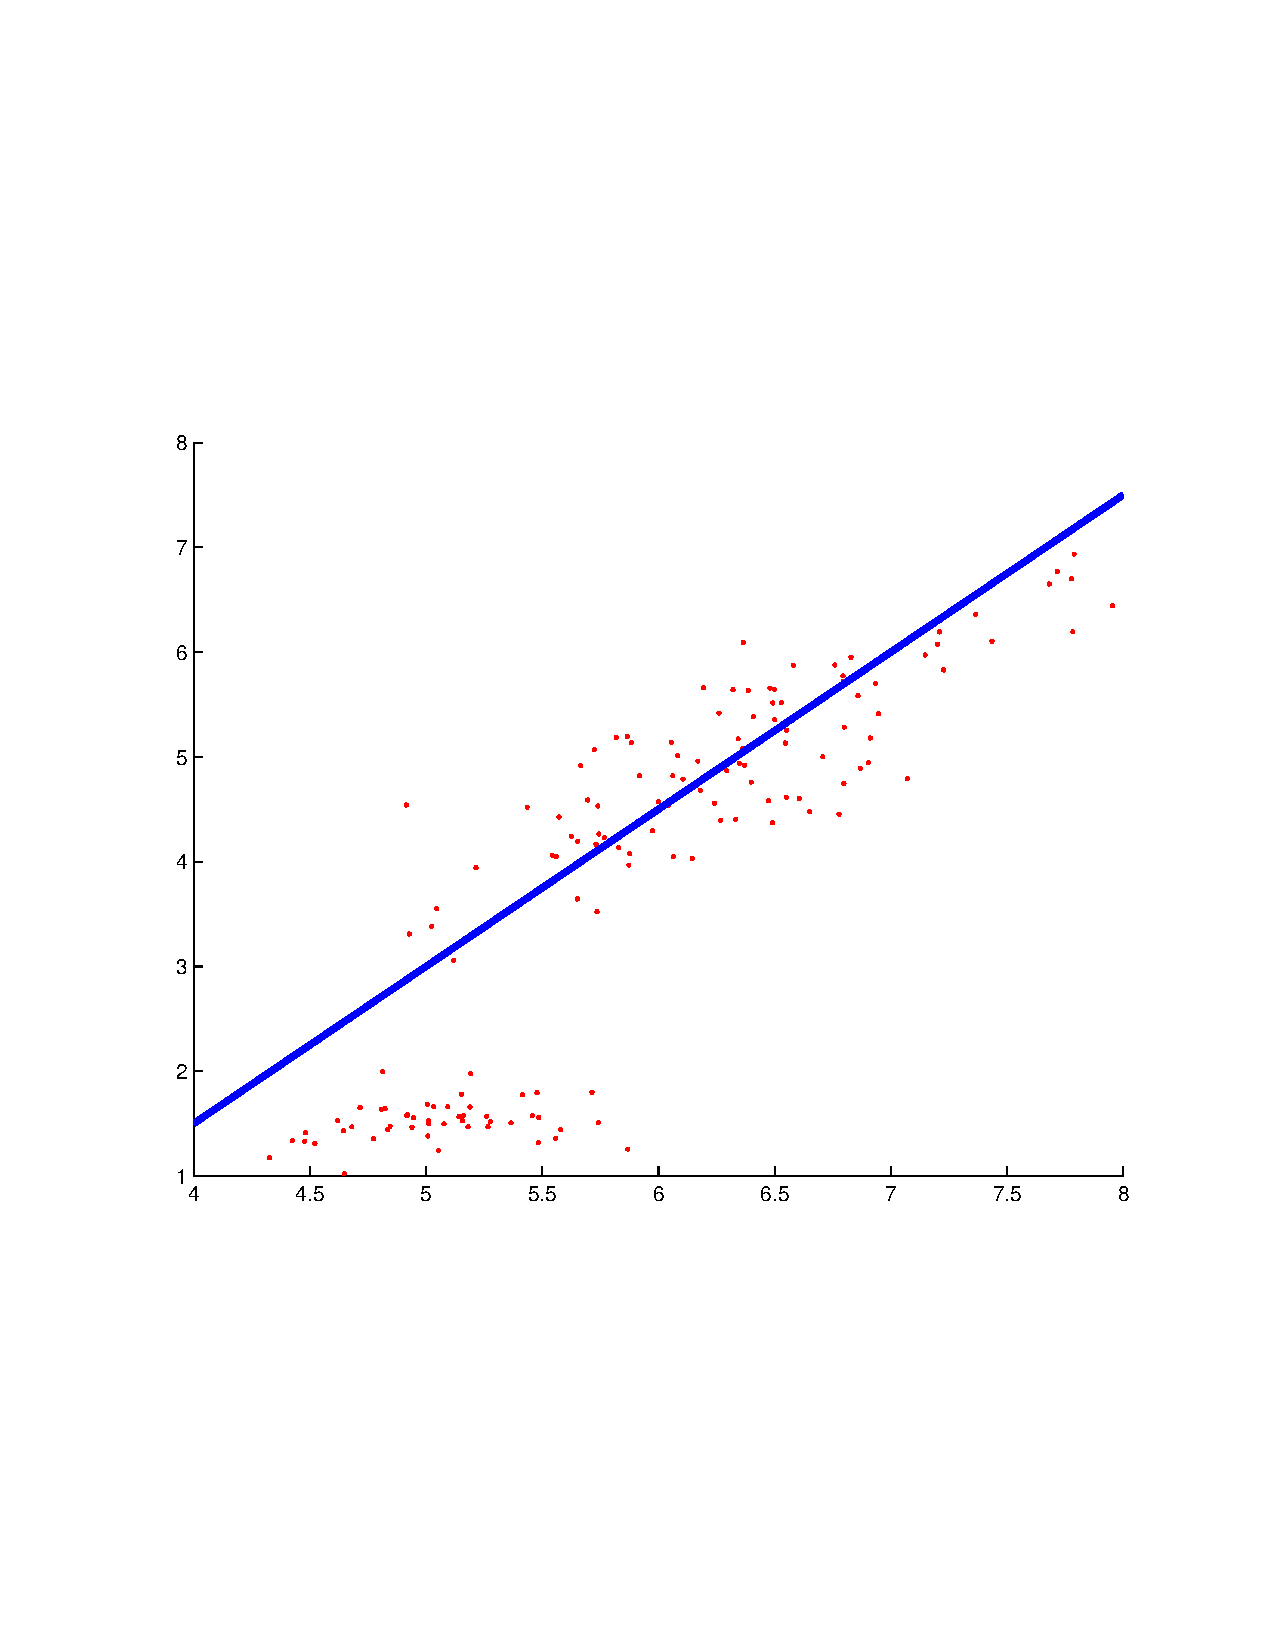
\includegraphics[width=.22\textwidth]{\figdir/problem4}

\subsection*{Problem 5: }

Using the following function:
\lstinputlisting{mydist.m}

I executed the command \texttt{plot(mydist(iris(1,:), iris))} to get the following plot:\\
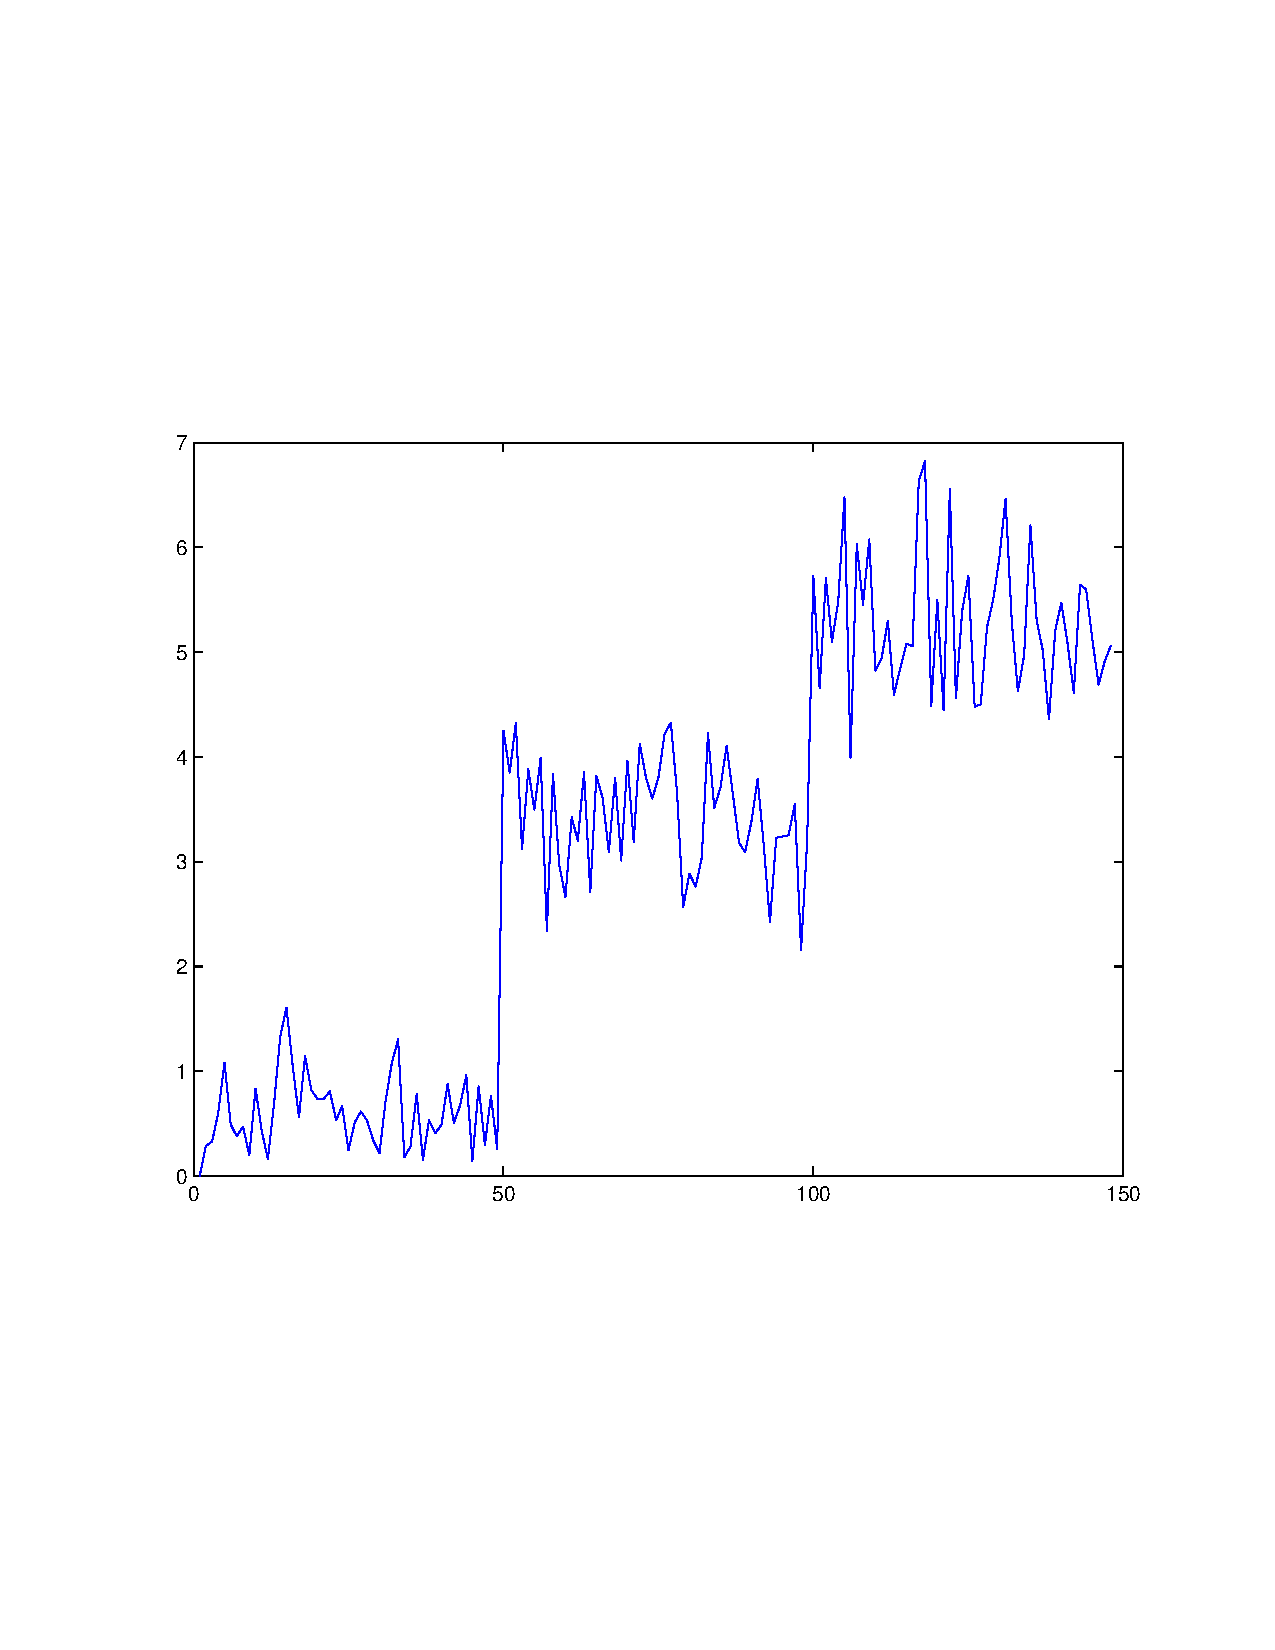
\includegraphics[width=.22\textwidth]{\figdir/problem5} \\

\end{document}
